% @Author: Qing Shi
% @LastEditTime: 2022/02/09

\documentclass[bachelor]{zufe}

\addbibresource{Reference.bib}

% % 使用中文编译 + XeLatex
% \usepackage[fontset=ubuntu]{ctex}

% 基本信息--------------------------------------------------------------------------------
% 在这里填写你的论文中文题目
\newcommand{\thesisTitle}{海岛环境对武学宗师成长的影响机理}
% 在这里填写你的论文英文题目
\newcommand{\thesisTitleEN}{Influence mechanism of island environment on the growth of martial arts masters}

% 若有副标题,则运行下一行的代码,若无副标题,则将下一行注释掉(在\haveSub{}最前面添加 % 号)
\haveSub{}

% 在这里填写你的论文中文副标题(没有只需注释掉\haveSub{}即可)
\newcommand{\thesisSubTitle}{基于桃花岛武学流派的研究}
% 在这里填写你的论文英文副标题(没有只需注释掉\haveSub{}即可)
\newcommand{\thesisSubTitleEN}{Research Based on Taohua island martial arts school}

% 在这里填写你的相关信息
\newcommand{\deptName}{信息管理与人工智能学院}
\newcommand{\majorName}{xxxx}
\newcommand{\yourName}{xx}
\newcommand{\yourStudentID}{180110910xxx}
\newcommand{\mentorName}{xxx}
\newcommand{\className}{xxx}
\newcommand{\Today}{2022年5月}
% 基本信息--------------------------------------------------------------------------------

% 文档开始
\begin{document}

% 封面,没有特殊情况不需要修改
% 封面
% 无特殊要求,不需要修改
% XelaTeX编译
\newcommand\dunderline[3][-1pt]{{%
  \setbox0=\hbox{#3}
  \ooalign{\copy0\cr\rule[\dimexpr#1-#2\relax]{\wd0}{#2}}}}

% Cover Page
\begin{titlepage}
  \makeatletter
  \@ifundefined{externalMentorName}{
    % 校内毕设封面顶部间距
    \vspace*{-20mm}
  }{
    % 校外毕设封面顶部间距
    \vspace*{13mm}
  }
  \centering

  
\includegraphics[width=3cm]{InitFile/schoolLogo.png}\\
  
\includegraphics[width=5cm, height=1cm]{InitFile/schoolName.png}

  \vspace*{10mm}
\begin{center}
  \zihao{1}\textbf{\ziju{0.12}\songti{本\hspace{5mm}科\hspace{5mm}生\hspace{5mm}毕\hspace{5mm}业\hspace{5mm}论\hspace{5mm}文(设计)}}

  \vspace{20mm}

  \xiaoer\textmd{\heiti{题目:}\thesisTitle}

  \vspace{5mm}
  \ifhaveSubTitle
  \begin{spacing}{1.2}
    \sanhao\selectfont{\textmd{\kaitigb{-----}\thesisSubTitle}}
  \end{spacing}
  \fi
  \vspace{30mm}

  \flushleft

  \makeatletter
  \@ifundefined{externalMentorName}{
    % 生成校内毕设封面字段
    \makeatother
    \begin{spacing}{1.8}
      \hspace{27mm}\songti\zihao{3}\selectfont{学生姓名:\dunderline[-10pt]{1pt}{\makebox[78mm][c]{\yourName}}}
      
      \hspace{27mm}\songti\zihao{3}\selectfont{学\hspace{11mm}号:\dunderline[-10pt]{1pt}{\makebox[78mm][c]{\yourStudentID}}}

      \hspace{27mm}\songti\zihao{3}\selectfont{指导教师:\dunderline[-10pt]{1pt}{\makebox[78mm][c]{\mentorName}}}
    
      \hspace{27mm}\songti\zihao{3}\selectfont{所在学院:\dunderline[-10pt]{1pt}{\makebox[78mm][c]{\deptName}}}

      \hspace{27mm}\songti\zihao{3}\selectfont{专业名称:\dunderline[-10pt]{1pt}{\makebox[78mm][c]{\majorName}}}
      
      \hspace{27mm}\songti\zihao{3}\selectfont{班\hspace{11mm}级:\dunderline[-10pt]{1pt}{\makebox[78mm][c]{\className}}}
    \end{spacing}
  }{
    % 生成校外毕设封面字段
    \makeatother
    \begin{spacing}{1.8}
      \hspace{19.4mm}\songti\zihao{3}\selectfont{学\hspace{19.6mm}院\hspace{3mm}:\dunderline[-10pt]{1pt}{\makebox[77.4mm][c]{\deptName}}}

      \hspace{19.4mm}\songti\zihao{3}\selectfont{专\hspace{19.6mm}业\hspace{3mm}:\dunderline[-10pt]{1pt}{\makebox[77.4mm][c]{\majorName}}}

      \hspace{19.4mm}\songti\zihao{3}\selectfont{学\hspace{2.8mm}生\hspace{2.8mm}姓\hspace{2.8mm}名\hspace{3mm}:\dunderline[-10pt]{1pt}{\makebox[77.4mm][c]{\yourName}}}

      \hspace{19.4mm}\songti\zihao{3}\selectfont{学\hspace{19.6mm}号\hspace{3mm}:\dunderline[-10pt]{1pt}{\makebox[77.4mm][c]{\yourStudentID}}}

      \hspace{19.4mm}\songti\zihao{3}\selectfont{指\hspace{2.8mm}导\hspace{2.8mm}教\hspace{2.8mm}师\hspace{3mm}:\dunderline[-10pt]{1pt}{\makebox[77.4mm][c]{\mentorName}}}

      \hspace{19.4mm}\songti\zihao{3}\selectfont{校外指导教师:\dunderline[-10pt]{1pt}{\makebox[77.4mm][c]{\externalMentorName}}}
    \end{spacing}
  }

  \vspace{25mm}
  \centering
  \zihao{4}\ziju{0.5}\xihei{\Today}
  \end{center}
\end{titlepage}



% 前置页面定义
\frontmatter

% 原创性声明,没有特殊情况不需要修改
% 原创性声明页
% 无特殊要求,不用修改

\fancypagestyle{originality}{
  % 页眉高度
  \setlength{\headheight}{10pt}

  % 页眉和页脚(页码)的格式设定
  \fancyhf{}
  \fancyhead[]{}

  % 页眉分割线稍微粗一些
  \renewcommand{\headrulewidth}{0pt}
}

\pagestyle{originality}
% \topskip=0pt

% % 圆形数字编号定义
% \newcommand{\circled}[2][]{\tikz[baseline=(char.base)]
%   {\node[shape = circle, draw, inner sep = 1pt]
%   (char) {\phantom{\ifblank{#1}{#2}{#1}}};
%   \node at (char.center) {\makebox[0pt][c]{#2}};}}
% \robustify{\circled}

% 设置行间距
\setlength{\parskip}{0.4em}
\renewcommand{\baselinestretch}{1.41}

% 顶部空白
\vspace*{-6mm}

% 原创性声明部分
\begin{center}
  \heiti\zihao{2}\textmd{声明及论文使用的授权}
\end{center}

\vspace{10mm}


% 本部分字号为小三
\zihao{-3}

本人郑重声明所呈交的论文是我个人在导师的指导下独立完成的。除了文中特别加以标注和致谢的地方外,论文中不包含其他人已经发表或撰写的研究成果。

\vspace{15mm}

\begin{flushright}
  论文作者签名:\hspace{75mm}年\hspace{8mm}月\hspace{8mm}日
\end{flushright}

\vspace{40mm}

% 使用授权声明部分

\zihao{-3}

本人同意浙江财经大学有关保留使用学位论文的规定,即:学校有权保留送交论文的复印件,允许论文被查阅和借阅;学校可以上网公布全部内容,可以采用影印、缩印或其他复制手段保存论文。

\vspace*{15mm}

\begin{flushright}
  论文作者签名:\hspace{75mm}年\hspace{8mm}月\hspace{8mm}日
\end{flushright}

\newpage


% 摘要(中英文):根据自身论文,修改摘要的Tex文件

% \fancypagestyle{abstract}{
%   % 页眉高度
%   \setlength{\headheight}{10pt}

%   % 页眉和页脚(页码)的格式设定
%   \fancyhf{}
%   \fancyhead[C]{\ziju{0.08}\songti\zihao{-5}{浙江财经大学本科生毕业论文(设计)}}

%   % 页眉分割线稍微粗一些
%   \renewcommand{\headrulewidth}{0.4pt}
% }

% \pagestyle{abstract}
% \topskip=0pt

% 中英文摘要章节
\zihao{-4}
\vspace*{-10mm}

\begin{center}
  \heiti\zihao{3}\textmd{\thesisTitle}
  \vspace{2mm}
  \ifhaveSubTitle
  \begin{spacing}{1.2}
    \sihao\selectfont{\textmd{\mystkaiti{-----}\thesisSubTitle}}
  \end{spacing}
  \fi
\end{center}

\vspace*{0mm}

{\let\clearpage\relax \chapter*{\textmd{}}}
% 加入目录
\addcontentsline{toc}{chapter}{摘~~~~要}
\setcounter{page}{1}

\vspace*{-12mm}

\setstretch{1.53}
\setlength{\parskip}{0em}

\textbf{\heiti\xiaosi{摘要:}}
% 中文摘要正文从这里开始-----------------------------------------------------------------
{\mystkaiti{
本文……生僻字:垚瑄。{\songti{正文默认字体为\textbackslash{}songti命令,与支持生僻字的{\mystsong{方正宋体}}略有区别,因此正文中宋体生僻字使用\textbackslash{}mystsong命令代替即可。如:\mystsong{垚瑄}}}。
\textcolor{blue}{摘要的内容要包括研究的目的、方法、结果和结论。计量单位一律换算成国际标准计量单位。除特殊情况外,数字一律用阿拉伯数字。中、英文摘要的内容应严格一致。}
}}

\vspace{1em}
\textbf{\heiti\xiaosi{关键词:}}
{\mystkaiti{
计算机科学与技术;算法;复杂度;深度学习;机器学习;可视化计算
}}
% \newpage

% 英文摘要章节
\vspace*{15mm}

\begin{spacing}{0.95}
  \centering
  \zihao{3}\textbf{\thesisTitleEN}
  \vspace{2mm}
  \ifhaveSubTitle
  \begin{spacing}{1.2}
    \sihao\selectfont{\textmd{{-----}\thesisSubTitleEN}}
  \end{spacing}
  \fi
\end{spacing}

\vspace*{0mm}

{\let\clearpage\relax \chapter*{\zihao{-3}\textmd{}\vskip -3bp}}
\addcontentsline{toc}{chapter}{Abstract}
\setcounter{page}{1}

\setstretch{1.53}
\setlength{\parskip}{0em}

\textbf{\heiti\xiaosi{Abstract: }}
% 英文摘要正文从这里开始-----------------------------------------------------------------
In order to study……


\textbf{\xiaosi{Key words:}}
Computer science and technology; Algorithm; Complexity; Deep learning; Machine learning; Visualization analysis
\newpage


% 目录,自动生成,没有特殊情况不需要修改
% 论文目录
% 没有特殊需要不用修改

%目录开始

% 调整目录行间距
\renewcommand{\baselinestretch}{1.35}
% 目录
\tableofcontents
\newpage


% 正文开始
\mainmatter
% 正文 22 磅的行距
\setlength{\parskip}{0em}
\renewcommand{\baselinestretch}{1.53}
% 修复脚注出现跨页的问题
\interfootnotelinepenalty=10000

% 引言,根据自身论文,修改引言的Tex文件
% 引言

\chapter{引~~~~言}
本文主要研究了

\textcolor{blue}{撰写引言部分,阅后删除}

% 章节模板,成文后将其注释掉即可
% 样例章节

% 章和引用示例-------------------------------------------------------------------------------------
\chapter{一级题目}

\section{二级题目}

正文······\cite{GB/T16159—1996} % 引用示例

\subsection{三级题目}

正文······\cite{Sobieski}
% 章和引用示例-------------------------------------------------------------------------------------

% 图示例----------------------------------------------------------------------------------------
\section{\textcolor{blue}{\underline{\underline{图-示例}}}}

\textcolor{blue}{图的位置:(1)图居中排列。
(2)图与上文之间应留一空行。
(3)图中若有附注,一律用阿拉伯数字按顺序编排,如注1,附注在图的下方。
}

\begin{figure}[htbp]
  \vspace{1mm} % 调整图片与上文的垂直距离
  \centering
  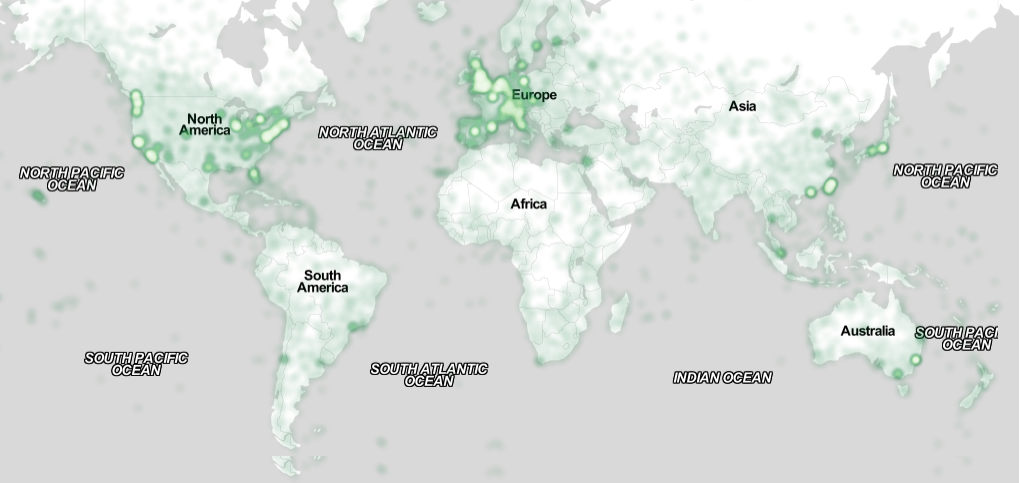
\includegraphics[width=300pt]{Images/map.png} % height 可以设置图片的高度, width 可以说设置图片的宽度
  \caption{样式1}\label{样式1} % label 用来在文中索引
  \vspace{-6mm} % 调整图片与下文的垂直距离
\end{figure}

下文······
% 图示例----------------------------------------------------------------------------------------

% 公式示例---------------------------------------------------------------------------------------
\section{\textcolor{blue}{\underline{\underline{公式-示例}}}}

\textcolor{blue}{公式标注应于该公式所在行的最右侧。对于较长的公式只可在符号处(+、-、*、/、$\leqslant$ $\geqslant$ 等)转行。在文中引用公式时,在标号前加“式”,如式(2-1)。}

% 公式上下不要空行,置于同一个段落下即可,否则上下距离会出现高度不一致的问题

\begin{equation}
    LRI=1\ ∕\ \sqrt{ 1 + {\left(\frac{{\mu}_{R}}{{\mu}_{s}}\right)^{2}}{\left(\frac{{\delta}_{R}}{{\delta}_{s}}\right)^{2}} }
\end{equation}
% 公式示例---------------------------------------------------------------------------------------

% 表示例----------------------------------------------------------------------------------------
\section{\textcolor{blue}{\underline{\underline{表-示例}}}}

\textcolor{blue}{{自动生成LaTeX表工具: \url{https://www.tablesgenerator.com/}}}

\begin{table}[htbp]
  \linespread{1.5}
  \zihao{5}
  \songti
  \centering
  \caption{物流的概念和范围}\label{物流的概念和范围}
  \begin{tabular}{|l|l|}
  \hline
  \multicolumn{1}{|c|}{本 质} & \multicolumn{1}{c|}{过  程}  \\ \hline
  途径或方法                     & 规划、实施、控制                   \\ \hline
  目标                        & 效率、成本效益                    \\ \hline
  活动或作业                     & 流动与储存                      \\ \hline
  处理对象                      & 原材料、在制品、产成品、相关信息           \\ \hline
  范围                        & 从原点(供应商)到终点(最终顾客)          \\ \hline
  目的或目标                     & 适应顾客的需求(产品、功能、数量、质量、时间、价格) \\ \hline
  \end{tabular}
\end{table}

% \begin{table}[htbp]
%   \linespread{1.5}
%   \zihao{5}
%   \songti
%   \centering
%   \caption{统计表}\label{统计表}
%   \begin{tabular}{|l|l|l|l|l|}
%   \hline
%   产品  & 产量    & 销量    & 产值   & 比重    \\ \hline
%   手机  & 11000 & 10000 & 500  & 50\%  \\ \hline
%   电视机 & 5500  & 5000  & 220  & 22\%  \\ \hline
%   计算机 & 1100  & 1000  & 280  & 28\%  \\ \hline
%   合计  & 17600 & 16000 & 1000 & 100\% \\ \hline
%   \end{tabular}
% \end{table}

\begin{table}[htbp]
  \linespread{1.5}
  \zihao{5}
  \songti
  \centering
  \caption{统计表}\label{统计表}
  % Please add the following required packages to your document preamble:
  % \usepackage{multirow}
  \begin{tabular}{|l|l|l|l|l|}
  \hline
  年度                    & 产品  & 产量    & 销量    & 产值  \\ \hline
  \multirow{2}{*}{2004} & 手机  & 11000 & 10000 & 500 \\ \cline{2-5} 
                      & 计算机 & 1100  & 1000  & 280 \\ \hline
  \multirow{2}{*}{2005} & 手机  & 16000 & 13000 & 550 \\ \cline{2-5} 
                      & 计算机 & 2100  & 1500  & 320 \\ \hline
  \end{tabular}
\end{table}
% 表示例----------------------------------------------------------------------------------------

% 伪代码示例------------------------------------------------------------------------------------

\section{\textcolor{blue}{\underline{\underline{伪代码-示例}}}}

\textcolor{blue}{修改 algorithmic 之间的代码就可以实现论文伪代码,已经考虑了伪代码跨页问题}
\begin{breakablealgorithm}
        \caption{Calculate $y = x^n$}
        \begin{algorithmic}[1] %每行显示行号
            \Require $n \geq 0 \vee x \neq 0$ 
            \Ensure  $y = x^n$
            \State $y \gets 1$
            \If{$n < 0$}
            \State $ X \gets 1 / x$
            \State $N \gets -n$
            \Else
            \State $X \gets x$
            \State $N \gets n$
            \EndIf
            \While{ $N \neq 0$ }
            \If{ $N$ is even }
            \State $X \gets x \times x$
            \State $N \gets N / 2$
            \Else[$N$ is odd]
            \State $y \gets y \times X$
            \State $N \gets N - 1$
            \EndIf
            \EndWhile
     \end{algorithmic}
    \end{breakablealgorithm}
% 伪代码示例------------------------------------------------------------------------------------

% 代码块示例------------------------------------------------------------------------------------
\section{\textcolor{blue}{\underline{\underline{代码块-示例}}}}
\textcolor{blue}{只写了 C++, Python, Java 三种语言的格式}

% C++ 代码引入 + 文件引入
\lstinputlisting[
style = C++,
caption = {test.cpp},
label = {test.cpp}
]{./papperCode/test.cpp}

% Java 代码引入 + 行内引入
\begin{lstlisting}[
style = Java,
caption = {test.jar},
label = {test.jar}
]
public class HelloWorld {
    public static void main(String[] args){
        System.out.println("Hello World!");
    }
}
\end{lstlisting}

% Python 代码引入 + 文件引入
\lstinputlisting[
style = Python,
caption = {test.py},
label = {test.py}
]{./papperCode/test.py}
% 代码块示例------------------------------------------------------------------------------------

% 在此插入章节
% 第一章
% 第一章
% 根据自身论文修改

\chapter{相关工作}
人工智能算法是时代的热点,在国内外都有许多学者进行研究。
\section{国内研究现状}
\subsection{机器学习}
\subsection{深度学习}

\section{国外研究现状}
\subsection{机器学习}
\subsection{深度学习}
% 第二章,第三章······

% 结论:根据自身论文,修改结论的Tex文件
%  结论

\unnumchapter{结~~~~论}
\renewcommand{\thechapter}{结论}

\ctexset{
  section/number = \arabic{section}
}

% 结论部分尽量不使用 \subsection 二级标题,只使用 \section 一级标题

% 这里插入一个参考文献,仅作参考
本文结论……。\cite{李成智2004飞行之梦}

\textcolor{blue}{结论作为毕业设计(论文)正文的最后部分单独排写,但不加章号。结论是对整个论文主要结果的总结。在结论中应明确指出本研究的创新点,对其应用前景和社会、经济价值等加以预测和评价,并指出今后进一步在本研究方向进行研究工作的展望与设想。结论部分的撰写应简明扼要,突出创新性。阅后删除此段。}

\textcolor{blue}{结论正文样式与文章正文相同:宋体、小四;行距:22 磅;间距段前段后均为 0 行。阅后删除此段。}

% 参考文献,无特殊要求不需要修改
% 添加参考文献请使用 BibTex 格式,添加至 Reference.bib 中,并在正文中使用 \cite{xxx}
% 成文后将% 参考文献


% 参考文献开始
\unnumchapter{参考文献}
\renewcommand{\thechapter}{参考文献}

% 设置参考文献字号为 5 号
\renewcommand*{\bibfont}{\zihao{5}}
% 设置参考文献各个项目之间的垂直距离为 0
\setlength{\bibitemsep}{0ex}
\setlength{\bibnamesep}{0ex}
\setlength{\bibinitsep}{0ex}
% 设置单倍行距
\renewcommand{\baselinestretch}{1.2}
% 设置参考文献顺序标签 `[1]` 与文献内容 `作者. 文献标题...` 的间距
\setlength{\biblabelsep}{0.5mm}
% 设置参考文献后文缩进为 0(与 Word 模板保持一致)
\renewcommand{\itemcmd}{
  \addvspace{\bibitemsep} % 恢复 \bibitemsep 的作用
  \mkgbnumlabel{\printfield{labelnumber}}
  \hspace{\biblabelsep}}
% 删除默认的「参考文献 / Reference」标题,使用上面定义的 section 标题

\textcolor{blue}{参考文献书写规范}

\textcolor{blue}{参考国家标准《信息与文献参考文献著录规则》【GB/T 7714—2015】,参考文献书写规范如下:}

\textcolor{blue}{\textbf{1. 文献类型和标识代码}}

\textcolor{blue}{普通图书:M}\qquad\textcolor{blue}{会议录:C}\qquad\textcolor{blue}{汇编:G}\qquad\textcolor{blue}{报纸:N}

\textcolor{blue}{期刊:J}\qquad\textcolor{blue}{学位论文:D}\qquad\textcolor{blue}{报告:R}\qquad\textcolor{blue}{标准:S}

\textcolor{blue}{专利:P}\qquad\textcolor{blue}{数据库:DB}\qquad\textcolor{blue}{计算机程序:CP}\qquad\textcolor{blue}{电子公告:EB}

\textcolor{blue}{档案:A}\qquad\textcolor{blue}{舆图:CM}\qquad\textcolor{blue}{数据集:DS}\qquad\textcolor{blue}{其他:Z}

\textcolor{blue}{\textbf{2. 不同类别文献书写规范要求}}

\textcolor{blue}{\textbf{期刊}}

\noindent\textcolor{blue}{[序号]主要责任者. 文献题名[J]. 刊名, 出版年份, 卷号(期号): 起止页码. }

\printbibliography [type=article,heading=none] 

\textcolor{blue}{\textbf{普通图书}}

\noindent\textcolor{blue}{[序号]主要责任者. 文献题名[M]. 出版地: 出版者, 出版年. 起止页码. }
\cite{Raymer1992Aircraft}

\printbibliography [keyword={book},heading=none] 

\textcolor{blue}{\textbf{会议论文集}}

\noindent\textcolor{blue}{[序号]析出责任者. 析出题名[A]. 见(英文用In): 主编. 论文集名[C]. (供选择项: 会议名, 会址, 开会年)出版地: 出版者, 出版年. 起止页码. }
\cite{sunpinyi}

\printbibliography [type=inproceedings,heading=none] 

\textcolor{blue}{\textbf{专著中析出的文献}}

\noindent\textcolor{blue}{[序号]析出责任者. 析出题名[A]. 见(英文用In): 专著责任者. 书名[M]. 出版地: 出版者, 出版年.起止页码. }
\cite{luoyun}

\printbibliography [type=inbook,heading=none] 

\textcolor{blue}{\textbf{学位论文}}

\noindent\textcolor{blue}{[序号]主要责任者. 文献题名[D]. 保存地: 保存单位, 年份. }
\cite{zhanghesheng}
\cite{Sobieski}

\printbibliography [keyword={thesis},heading=none] 

\textcolor{blue}{\textbf{报告}}

\noindent\textcolor{blue}{[序号]主要责任者. 文献题名[R]. 报告地: 报告会主办单位, 年份. }
\cite{fengxiqiao}
\cite{Sobieszczanski}

\printbibliography [keyword={techreport},heading=none] 

\textcolor{blue}{\textbf{专利文献}}

\noindent\textcolor{blue}{[序号]专利所有者. 专利题名[P]. 专利国别: 专利号, 发布日期. }
\cite{jiangxizhou}

\printbibliography [type=patent,heading=none] 

\textcolor{blue}{\textbf{国际、国家标准}}

\noindent\textcolor{blue}{[序号]标准代号. 标准名称[S]. 出版地: 出版者, 出版年. }
\cite{GB/T16159—1996}

\printbibliography [keyword={standard},heading=none] 

\textcolor{blue}{\textbf{报纸文章}}

\noindent\textcolor{blue}{[序号]主要责任者. 文献题名[N]. 报纸名, 出版年, 月(日): 版次. }
\cite{xiexide}

\printbibliography [keyword={newspaper},heading=none] 

\textcolor{blue}{\textbf{电子文献}}

\noindent\textcolor{blue}{[序号]主要责任者. 电子文献题名[文献类型/载体类型]. 电子文献的出版或可获得地址(电子文献地址用文字表述), 发表或更新日期/引用日期(任选). }
\cite{yaoboyuan}

\printbibliography [keyword={online},heading=none] 

\textcolor{blue}{关于参考文献的未尽事项可参考国家标准《信息与文献参考文献著录规则》(GB/T 7714—2015)}

%输出所有的参考文献
%\printbibliography[heading=none]
注释掉即可
% 参考文献


% 参考文献开始
\unnumchapter{参考文献}
\renewcommand{\thechapter}{参考文献}

% 设置参考文献字号为 5 号
\renewcommand*{\bibfont}{\zihao{5}}
% 设置参考文献各个项目之间的垂直距离为 0
\setlength{\bibitemsep}{0ex}
\setlength{\bibnamesep}{0ex}
\setlength{\bibinitsep}{0ex}
% 设置单倍行距
\renewcommand{\baselinestretch}{1.2}
% 设置参考文献顺序标签 `[1]` 与文献内容 `作者. 文献标题...` 的间距
\setlength{\biblabelsep}{0.5mm}
% 设置参考文献后文缩进为 0(与 Word 模板保持一致)
\renewcommand{\itemcmd}{
  \addvspace{\bibitemsep} % 恢复 \bibitemsep 的作用
  \mkgbnumlabel{\printfield{labelnumber}}
  \hspace{\biblabelsep}}
% 删除默认的「参考文献 / Reference」标题,使用上面定义的 section 标题

\textcolor{blue}{参考文献书写规范}

\textcolor{blue}{参考国家标准《信息与文献参考文献著录规则》【GB/T 7714—2015】,参考文献书写规范如下:}

\textcolor{blue}{\textbf{1. 文献类型和标识代码}}

\textcolor{blue}{普通图书:M}\qquad\textcolor{blue}{会议录:C}\qquad\textcolor{blue}{汇编:G}\qquad\textcolor{blue}{报纸:N}

\textcolor{blue}{期刊:J}\qquad\textcolor{blue}{学位论文:D}\qquad\textcolor{blue}{报告:R}\qquad\textcolor{blue}{标准:S}

\textcolor{blue}{专利:P}\qquad\textcolor{blue}{数据库:DB}\qquad\textcolor{blue}{计算机程序:CP}\qquad\textcolor{blue}{电子公告:EB}

\textcolor{blue}{档案:A}\qquad\textcolor{blue}{舆图:CM}\qquad\textcolor{blue}{数据集:DS}\qquad\textcolor{blue}{其他:Z}

\textcolor{blue}{\textbf{2. 不同类别文献书写规范要求}}

\textcolor{blue}{\textbf{期刊}}

\noindent\textcolor{blue}{[序号]主要责任者. 文献题名[J]. 刊名, 出版年份, 卷号(期号): 起止页码. }

\printbibliography [type=article,heading=none] 

\textcolor{blue}{\textbf{普通图书}}

\noindent\textcolor{blue}{[序号]主要责任者. 文献题名[M]. 出版地: 出版者, 出版年. 起止页码. }
\cite{Raymer1992Aircraft}

\printbibliography [keyword={book},heading=none] 

\textcolor{blue}{\textbf{会议论文集}}

\noindent\textcolor{blue}{[序号]析出责任者. 析出题名[A]. 见(英文用In): 主编. 论文集名[C]. (供选择项: 会议名, 会址, 开会年)出版地: 出版者, 出版年. 起止页码. }
\cite{sunpinyi}

\printbibliography [type=inproceedings,heading=none] 

\textcolor{blue}{\textbf{专著中析出的文献}}

\noindent\textcolor{blue}{[序号]析出责任者. 析出题名[A]. 见(英文用In): 专著责任者. 书名[M]. 出版地: 出版者, 出版年.起止页码. }
\cite{luoyun}

\printbibliography [type=inbook,heading=none] 

\textcolor{blue}{\textbf{学位论文}}

\noindent\textcolor{blue}{[序号]主要责任者. 文献题名[D]. 保存地: 保存单位, 年份. }
\cite{zhanghesheng}
\cite{Sobieski}

\printbibliography [keyword={thesis},heading=none] 

\textcolor{blue}{\textbf{报告}}

\noindent\textcolor{blue}{[序号]主要责任者. 文献题名[R]. 报告地: 报告会主办单位, 年份. }
\cite{fengxiqiao}
\cite{Sobieszczanski}

\printbibliography [keyword={techreport},heading=none] 

\textcolor{blue}{\textbf{专利文献}}

\noindent\textcolor{blue}{[序号]专利所有者. 专利题名[P]. 专利国别: 专利号, 发布日期. }
\cite{jiangxizhou}

\printbibliography [type=patent,heading=none] 

\textcolor{blue}{\textbf{国际、国家标准}}

\noindent\textcolor{blue}{[序号]标准代号. 标准名称[S]. 出版地: 出版者, 出版年. }
\cite{GB/T16159—1996}

\printbibliography [keyword={standard},heading=none] 

\textcolor{blue}{\textbf{报纸文章}}

\noindent\textcolor{blue}{[序号]主要责任者. 文献题名[N]. 报纸名, 出版年, 月(日): 版次. }
\cite{xiexide}

\printbibliography [keyword={newspaper},heading=none] 

\textcolor{blue}{\textbf{电子文献}}

\noindent\textcolor{blue}{[序号]主要责任者. 电子文献题名[文献类型/载体类型]. 电子文献的出版或可获得地址(电子文献地址用文字表述), 发表或更新日期/引用日期(任选). }
\cite{yaoboyuan}

\printbibliography [keyword={online},heading=none] 

\textcolor{blue}{关于参考文献的未尽事项可参考国家标准《信息与文献参考文献著录规则》(GB/T 7714—2015)}

%输出所有的参考文献
%\printbibliography[heading=none]

% 参考文献


% 参考文献开始
\unnumchapter{参考文献}
\renewcommand{\thechapter}{参考文献}

% 设置参考文献字号为 5 号
\renewcommand*{\bibfont}{\zihao{5}}
% 设置参考文献各个项目之间的垂直距离为 0
\setlength{\bibitemsep}{0ex}
\setlength{\bibnamesep}{0ex}
\setlength{\bibinitsep}{0ex}
% 设置单倍行距
\renewcommand{\baselinestretch}{1.2}
% 设置参考文献顺序标签 `[1]` 与文献内容 `作者. 文献标题...` 的间距
\setlength{\biblabelsep}{0.5mm}
% 设置参考文献后文缩进为 0(与 Word 模板保持一致)
\renewcommand{\itemcmd}{
  \addvspace{\bibitemsep} % 恢复 \bibitemsep 的作用
  \mkgbnumlabel{\printfield{labelnumber}}
  \hspace{\biblabelsep}}
% 删除默认的「参考文献 / Reference」标题,使用上面定义的 section 标题

% \textcolor{blue}{参考文献书写规范}

% \textcolor{blue}{参考国家标准《信息与文献参考文献著录规则》【GB/T 7714—2015】,参考文献书写规范如下:}

% \textcolor{blue}{\textbf{1. 文献类型和标识代码}}

% \textcolor{blue}{普通图书:M}\qquad\textcolor{blue}{会议录:C}\qquad\textcolor{blue}{汇编:G}\qquad\textcolor{blue}{报纸:N}

% \textcolor{blue}{期刊:J}\qquad\textcolor{blue}{学位论文:D}\qquad\textcolor{blue}{报告:R}\qquad\textcolor{blue}{标准:S}

% \textcolor{blue}{专利:P}\qquad\textcolor{blue}{数据库:DB}\qquad\textcolor{blue}{计算机程序:CP}\qquad\textcolor{blue}{电子公告:EB}

% \textcolor{blue}{档案:A}\qquad\textcolor{blue}{舆图:CM}\qquad\textcolor{blue}{数据集:DS}\qquad\textcolor{blue}{其他:Z}

% \textcolor{blue}{\textbf{2. 不同类别文献书写规范要求}}

% \textcolor{blue}{\textbf{期刊}}

% \noindent\textcolor{blue}{[序号]主要责任者. 文献题名[J]. 刊名, 出版年份, 卷号(期号): 起止页码. }

% \printbibliography [type=article,heading=none] 

% \textcolor{blue}{\textbf{普通图书}}

% \noindent\textcolor{blue}{[序号]主要责任者. 文献题名[M]. 出版地: 出版者, 出版年. 起止页码. }
% \cite{Raymer1992Aircraft}

% \printbibliography [keyword={book},heading=none] 

% \textcolor{blue}{\textbf{会议论文集}}

% \noindent\textcolor{blue}{[序号]析出责任者. 析出题名[A]. 见(英文用In): 主编. 论文集名[C]. (供选择项: 会议名, 会址, 开会年)出版地: 出版者, 出版年. 起止页码. }
% \cite{sunpinyi}

% \printbibliography [type=inproceedings,heading=none] 

% \textcolor{blue}{\textbf{专著中析出的文献}}

% \noindent\textcolor{blue}{[序号]析出责任者. 析出题名[A]. 见(英文用In): 专著责任者. 书名[M]. 出版地: 出版者, 出版年.起止页码. }
% \cite{luoyun}

% \printbibliography [type=inbook,heading=none] 

% \textcolor{blue}{\textbf{学位论文}}

% \noindent\textcolor{blue}{[序号]主要责任者. 文献题名[D]. 保存地: 保存单位, 年份. }
% \cite{zhanghesheng}
% \cite{Sobieski}

% \printbibliography [keyword={thesis},heading=none] 

% \textcolor{blue}{\textbf{报告}}

% \noindent\textcolor{blue}{[序号]主要责任者. 文献题名[R]. 报告地: 报告会主办单位, 年份. }
% \cite{fengxiqiao}
% \cite{Sobieszczanski}

% \printbibliography [keyword={techreport},heading=none] 

% \textcolor{blue}{\textbf{专利文献}}

% \noindent\textcolor{blue}{[序号]专利所有者. 专利题名[P]. 专利国别: 专利号, 发布日期. }
% \cite{jiangxizhou}

% \printbibliography [type=patent,heading=none] 

% \textcolor{blue}{\textbf{国际、国家标准}}

% \noindent\textcolor{blue}{[序号]标准代号. 标准名称[S]. 出版地: 出版者, 出版年. }
% \cite{GB/T16159—1996}

% \printbibliography [keyword={standard},heading=none] 

% \textcolor{blue}{\textbf{报纸文章}}

% \noindent\textcolor{blue}{[序号]主要责任者. 文献题名[N]. 报纸名, 出版年, 月(日): 版次. }
% \cite{xiexide}

% \printbibliography [keyword={newspaper},heading=none] 

% \textcolor{blue}{\textbf{电子文献}}

% \noindent\textcolor{blue}{[序号]主要责任者. 电子文献题名[文献类型/载体类型]. 电子文献的出版或可获得地址(电子文献地址用文字表述), 发表或更新日期/引用日期(任选). }
% \cite{yaoboyuan}

% \printbibliography [keyword={online},heading=none] 

% \textcolor{blue}{关于参考文献的未尽事项可参考国家标准《信息与文献参考文献著录规则》(GB/T 7714—2015)}

%输出所有的参考文献
\printbibliography[heading=none]


% 附录:根据自身论文,修改附录的Tex文件(补充论文,不是必须)
% 附录

\unnumchapter{附录A~~~~附录内容的名称}
\renewcommand{\thechapter}{附录}

% % 设置附录编号格式
% \ctexset{
%   section/number = 附录\Alph{section}
% }

% 附录相关内容…

% % 这里示范一下添加多个附录的方法:

% \section{\LaTeX 环境的安装}
% \LaTeX 环境的安装。

% \section{使用说明}
% 使用说明。

\textcolor{blue}{以下内容可放在附录之内:
1.正文内过于冗长的公式推导;
2.方便他人阅读所需的辅助性数学工具或表格;
3.重复性数据和图表;
4.论文使用的主要符号的意义和单位;
5.程序说明和程序全文;
6.调研报告。
}

\textcolor{blue}{这部分内容可省略(如果省略,删去此页)。阅后删除此段。}


% 致谢:根据自身要求,修改致谢的Tex文件
% 致谢

\unnumchapter{致~~~~谢}
\renewcommand{\thechapter}{致谢}

\ctexset{
  section/number = \arabic{section}
}

% 致谢部分尽量不使用 \subsection 二级标题,只使用 \section 一级标题

值此论文完成之际,首先向我的导师……

\textcolor{blue}{致谢正文样式与文章正文相同:宋体、小四;行距:22 磅;间距段前段后均为 0 行。阅后删除此段。}

\end{document}
